\chapter{Ergebnisse}
%  Hauptergebnisse hier! 
%  Je Aufnahme:  Beschreibung der Laufzeiten verschiedener funktionen (lichtmenge berechnen, frames berechnen)\\
%                Reale Gesamtdauer einer einzelnen Langzeitaufnahme sowie der gesammten Beleuchtung \\
%  Ergebnisse mit lenovo (fuer chrome-cat evtl MBP):
   In diesem Kapitel wird gezeigt wie sich das Beleuchtungsverfahren, dessen einzelne Teilaspekte in Abschnitt \ref{evaluation} bereits getrennt evaluiert wurden, in der Praxis verhält.
   Hierzu wurden zwei Szenen mit den folgenden Eigenschaften ausgewählt:
   \begin{itemize}
    \item{Szene 1: stark spiegelnde und transparenten Objekte ($r_s=$ 3cm)}
    \item{ Szene 2: gemischte Szene mit Schatten ($r_s=$ 5 cm)}
   \end{itemize}
   
  Anhand Szene 1 (siehe Abschnitt \ref{szene1}) soll gezeigt werden, dass das Beleuchtungsverfahren funktioniert und es damit möglich ist, eine einfallende Beleuchtung mit einer hohen Auflösung zu erzeugen.
  Dazu wurde sie von allen Richtungen beleuchtet, die mit dem Laptop und der Tracking-Stage erreicht werden konnten.
  Damit die einzelnen Teilbeleuchtungen dabei möglichst schnell erzeugt werden können wurde eine kurze HDR-Sequenz gewählt und der Dynamikbereich der Environment-Map reduziert.
  
  Mit Szene 2 (siehe Abschnitt \ref{szene2}) hingegen soll demonstriert werden, dass eine korrekte Beleuchtung nur dann möglich ist, wenn man lange HDR-Sequenzen verwendet. 
  Eine vollständige HDR-Beleuchtung mit langen HDR-Sequenzen (150 Frames und mehr) würde jedoch viele Stunden dauern und ist damit nicht mehr praktisch anwendbar. 
  Für Szene 2 wurde darum eine synthetische Environment-Map verwendet, und nur eine einzige Teilbeleuchtung erzeugt.
   

\section {Ergebnis: Szene 1} \label{szene1}

   Für Szene 1 wurde eine Environment-Map mit reduziertem Kontrast (etwa 200:1) verwendet, und eine HDR-Sequenz der Länge 20 gewählt.
   Damit konnte für die DSLR-Aufnahmen eine Belichtungszeit von  1.6 Sekunden gewählt werden, wodurch sich eine Teilbeleuchtung im Bestfall unter 10 Sekunden erzeugen ließ.
   
   Die Toleranzen wurde so eingestellt, dass der Bildschirmabstand $r_l=$50 cm vom Benutzer  auf $\pm$5 cm genau eingehalten werden muss. 
   In so gut wie allen Teilbeleuchtungen konnte der Drift des Bildschirmzentrums geringer als 1 cm gehalten werden.
   Für die allerobersten Positionen, bei denen der Bildschirm mit ausgestreckten Armen gehalten werden muss, ware es jedoch notwendig 2 cm Drift zu erlauben.
   Für den Winkel zwischen Bildschirmnormalen und dem Vektor $\vec{f}$ wurden maximal  $5^\circ$ zugelassen; die allerunterste Reihe konnte jedoch nur bei einem Winkel von $7^\circ$ erreicht werden.
   Insgesamt wurden 78 Teilbeleuchtungen erzeugt, wobei der ungenutzte Rand 23x24 Pixel groß war. Die Verwendete Anzeigefläche betrug damit 1320x720 Pixel.
   
   Zur Beleuchtung wurde die in Abbildung \ref{fig:result_cubemap} gezeigte Environment-Map gewählt.
   Die Bildschirmpositionen der einzelnen Teilbeleuchtungen sind ebenfalls in Abbildung \ref{fig:result_cubemap} dargestellt. 

   \begin{figure}[H]
    \centering
     \includegraphics[width=0.9\textwidth]{../graphics/ergebnisse/cubemap_grace_ldr_small.jpg}
     \includegraphics[width=0.9\textwidth]{../graphics/ergebnisse/cubemap_used_all_small.png}
    \caption[Ergebnis: Szene 1 (Cube-Map)]{\textbf{Oben:} Die für Szene 1 verwendete ``Grace''-Environment-Map entstammt der Debevec Light Probe Gallery \cite{lightprobe_gallery}. 
   Der Dynamikbereich wurde mit dem Adaptive-Logarithmic-Tonemapping Verfahren \cite{Drago_2003}  auf etwa 200:1 reduziert. Die Auflösung jeder Textur beträgt 1000x1000 Pixel.
 \textbf{Unten:} Die Bildschirmpositionen und Überlappungen aller 78 Teilbeleuchtungen.
}
    \label{fig:result_cubemap}
   \end{figure}

  Abbildung \ref{fig:result_positions} zeigt die Bildschirmzentren aller Teilbeleuchtung als 3D-Plot. Die Farbe gibt dabei den Index $i$ der aufsteigend nummerierten Teilbeleuchtungen an. 
   Man kann erkennen, dass der Backdrop als erstes hergestellt wurde (schwarz).
   Anschließend wurde der Bildschirm kreisförmig um die Szene, hin und her bewegt und die obere Hälfte der einfallen Beleuchtung von unten nach oben erzeugt.
   Die untersten Teilbeleuchtungen (gelb) sind als letztes entstanden.
   
    \begin{figure}[H]
    \centering
    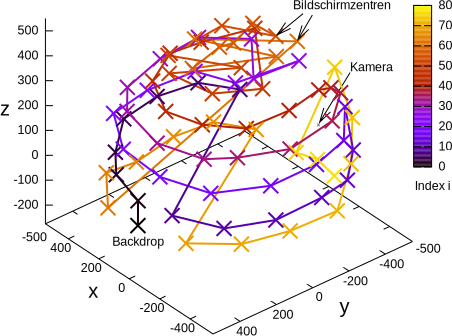
\includegraphics[width=0.55\textwidth]{../graphics/ergebnisse/positions.svg}
    \caption[Ergebnis: Szene 1 (Bildschirmpositionen als 3D-Plot)]{Die Position des Bildschirmzentrums ($\vec{f}$) bei jeder der 78 Teilbeleuchtungen von Szene 1 (in Millimeter). Die Farbe der Linie gibt die Reihenfolge an, in der die Beleuchtungen erzeugt wurden.}
    \label{fig:result_positions}
   \end{figure}


\pagebreak
   \begin{figure}[H]
    \centering
    \includegraphics[width=0.7\textwidth]{../graphics/ergebnisse/result_all_extended.jpg}
    \caption[Ergebnis: Szene 1]{ Szene 1 wurde mit der Environment-Map aus Abbildung \ref{fig:result_cubemap} beleuchtet. Das Ergebnis wurde aus insgesamt 78 Teilbeleuchtungen zusammengesetzt.  
    Die schwarzen Flächen sind Positionen, die mit dem Laptop nicht erreicht werden konnten (unteres Drittel der Environment-Map).
    Es ist gut zu erkennen das die meisten der Teilbeleuchtungen, trotz einer hohen Winkeltoleranz von $7^\circ$, eine optisch zusammenhängende  Lichtfläche erzeugen. Überlappungen werden korrekt behandelt, wenn der Bildschirm ruhig gehalten wird.
    Im Bild sieht man jedoch auch mehrere Teilbeleuchtungen, die zu dunkel oder verrutscht sind.
    Diese Artefakte werden in  Abbildung \ref{fig:result_discussion} genauer untersucht.
}

    \label{fig:result}
   \end{figure}


   \begin{table}[h]
    \begin{tabular}{|l|l|}
   \hline 
    \multicolumn{2}{|c|} { Dauer der Beleuchtung } \\
     \hline
     Anzahl Teilbeleuchtungen  & 78 \\
     Benötigte Zeit (gesamt) & 95 Minuten \\
     Benötigte Zeit (pro Teilbeleuchtung) & 73 Sekunden \\
     \hline
    \multicolumn{2}{|c|} { Durchschnittliche Laufzeiten } \\
     \hline
      Projektion $P$ (Cube-Map auf Bildschirm) & 64.32 ms \\ 
      Projektion $P^{-1}$ (Bildschirm auf Cube-Map) & 77.37 ms\\
      HDR-Algorithmus  & 796.08 ms  \\
      Positionsberechnung & 4.82 ms  \\
     \hline
        
    \end{tabular}
    \caption[Ergebnis: Szene 1 (Laufzeiten)]{ Dauer der Beleuchtung von Szene 1 und durchschnittliche Laufzeiten. }
    \label{result_stats}
   \end{table}




   \begin{figure}[H]
    \centering
      \includegraphics[width=0.6\textwidth]{../graphics/ergebnisse/result_all_extended_annotated.png} 
    \caption[Ergebnis: Szene 1 (Artefakte)]{ 
     Erklärung der Artefakte die im Ergebnisbild der Szene 1 zu sehen sind:
     \begin{itemize}
       \item{\textbf{A}:} Unerreichbare Position: Der Laptop kann nicht an diese Positionen bewegt werden, da die Fiducials der Tracking-Stage hier außerhalb des Webcamfrustums liegen.
       \item{\textbf{B}:} Position der DSLR-Kamera: Hier kann keine Beleuchtung erzeugt werden, da das Blickfeld der Kamera nicht verdeckt werden darf.
       \item{\textbf{C}:} Hier spiegeln sich die Fiducials: Sie sind als schwaches, rotes Rauschen sichtbar, weil  sie vom Bildschirm beleuchtet werden. 
       \item{\textbf{D}:} Oberste Bildschirmposition: Der Bildschirm musste hier mit ausgestreckten Armen gehalten werden, wodurch es su einem stärkeren Drift kam.
      \item{\textbf{E}:} Die Kamera hat sich zwischen den Aufnahmen minimal verschoben: Der schwarze Rand sollte hier nicht sein.
       \item{\textbf{F}:} Überlappung im Backdrop: Verursacht  durch eine ungenaue Position oder ein Drift (als heller Streifen in Abbildung \ref{fig:result} sichtbar).
       \item{\textbf{G}:} Diffuse Flächen sind verrauscht und zu dunkel: Der Dynamikbereich der DSLR-Kamera ist zu klein. Die Intensität des Lichts, das an diesen Stellen bei einer Teilbeleuchtung reflektiert wird, ist zu niedrig und kann deshalb nicht korrekt gemessen werden. 
    \item{\textbf{H}:} Teilbeleuchtungen mit zu niedriger Intensität: Verursacht durch Probleme bei der Shuttersteuerung; der DSLR-Shutter löste zu spät aus.
     \end{itemize}
     

     }
    \label{fig:result_discussion}
   \end{figure}
 
   \begin{figure}[H]
    \centering
    \begin{tabular}{c}
      \includegraphics[width=0.7\textwidth]{../graphics/ergebnisse/result_part_cubemap.png}
\\
      \includegraphics[width=0.24\textwidth]{../graphics/ergebnisse/result_part_67.png}
      \includegraphics[width=0.24\textwidth]{../graphics/ergebnisse/result_part_66.png}
      \includegraphics[width=0.24\textwidth]{../graphics/ergebnisse/result_part_65.png}
      \includegraphics[width=0.24\textwidth]{../graphics/ergebnisse/result_part_64.png}
 \\
      \includegraphics[width=0.24\textwidth]{../graphics/ergebnisse/result_screen_67.jpg}
      \includegraphics[width=0.24\textwidth]{../graphics/ergebnisse/result_screen_66.jpg}
      \includegraphics[width=0.24\textwidth]{../graphics/ergebnisse/result_screen_65.jpg}
      \includegraphics[width=0.24\textwidth]{../graphics/ergebnisse/result_screen_64.jpg}
 
    \end{tabular}
    \caption[Ergebnis: Szene 1 (vier Teilbeleuchtungen)]{ Die 64.-67. Teilbeleuchtung. \textbf{Oben:} Die Bildschirmpositionen als Cube-Map; die Beleuchtungen wurden von rechts nach links erzeugt. \textbf{Mitte:} Aufnahme $T_i$ (Darkframe nicht abgezogen). Die leuchtenden Fiducials, sowie der hohe Schwarzwert des Bildschirms sind zu erkennen.
   \textbf{Unten:} Die Strahldichteverteilung $L_r$ der Teilbeleuchtungen. Durch die Überlappungen bleiben teilweise große Bereiche der Bildschirmfläche ungenutzt. }
    \label{fig:result_parts}
   \end{figure}



   \begin{figure}[h]
    \centering
    \begin{tabular}{cc}
     \includegraphics[width=0.40\textwidth]{../graphics/ergebnisse/result_all_extended_small.jpg} 
    &
     \includegraphics[width=0.40\textwidth]{../graphics/ergebnisse/cat_compare_small.jpg}
    \\ 
    a) Ergebnis & b) reale Beleuchtung \\
    \end{tabular}
    \caption[Ergebnis: Szene 1 (Vergleich) ]{ Vergleich zwischen dem Ergebnis (links) und einer echten Beleuchtung (rechts).
      Man sieht das die weißen, diffusen Würfelaugen unter Einfluss einer realen Beleuchtung deutlich heller sind als im Ergebnis (siehe Artefakt \textbf{G} in Abbildung \ref{fig:result_discussion}). }

    \label{fig:result_comparison}
   \end{figure}

   \begin{figure}[h]
    \centering
    \begin{tabular}{cc}
     \includegraphics[width=0.40\textwidth]{../graphics/ergebnisse/result_reflective_extended_small.jpg}
    &
     \includegraphics[width=0.40\textwidth]{../graphics/ergebnisse/result_background_small.jpg}
    \\
    a) ohne Hintergrund & a) nur Hintergrund \\
    \end{tabular}
    \caption[Ergebnis: Szene 1 (Hintergrund) ]{ Die Szene lässt sich ganz einfach vom Hintergrund trennen, indem nur bestimmte Teilbeleuchtungen zusammengeführt werden. Abbildung \textbf{a)} zeigt Szene 1 ohne Hintergrund,  Abbildung \textbf{b)} hingegen zeigt nur den Hintergrund. }
    \label{fig:result_background}
   \end{figure}




\section {Ergebnis: Szene 2} \label{szene2}
   Szene 2 besteht aus verschiedenen diffusen, glänzenden und transluzenten Objekten, die so angeordnet sind, dass Schatten und Kaustiken gut sichtbar gemacht werden können.
   
   Für die Beleuchtung wurden zwei synthetische Environment-Maps gewählt. Beide bestehen aus einer einzigen kleinen, punktförmige Lichtquelle (weiß), die bei 50cm Entfernung etwa 2cm auf dem Bildschirm einnimmt.
   In der ersten Environment-Maps ist die Lichtquelle zusätzlich von einer großen Flächenlichtquelle (grün) mit niedriger Intensität umgeben.
   Die relative Strahldichte der Punktlichtquelle ist  500-mal größer als die der Flächenlichtquelle - das Kontrastverhältnis der Beleuchtung beträgt also 500:1.
   Die Länge der HDR-Sequenz wurde mit 160 Frames so groß gewählt, dass das dieses  Kontrastverhältnis auch dargestellt werden kann. 
   
   Abbildung \ref{fig:szene2} zeigt Szene 2 unter beiden Beleuchtungen.
   Hierzu wurde jeweils einer HDR-Aufnahme aus drei Belichtungen (10/20/30 s) rekonstruiert.
   Es ist deutlich zu erkennen, dass auch Lichtquellen mit einer geringen Intensität einen signifikanten Einfluss auf das Erscheinungsbild haben können, wenn sie eine große Fläche einnehmen.
  Da eine echte Umgebungsbeleuchtungen sowohl große Flächen mit geringer Intensität, als auch kleine Flächen mit sehr hoher Intensität besitzt, kann man sie nur mit einer HDR-Beleuchtung wahrheitsgetreu erzeugen.
  Eine vollständige HDR-Beleuchtung ist mit dem in dieser Arbeit vorgestellten System aufgrund der langen HDR-Sequenzen leider nur unter großem Zeitaufwand möglich.   
 
    \begin{figure}[H]
    \centering
    \begin{tabular}{c}
      \includegraphics[width=0.1\textwidth]{../graphics/ergebnisse/hdr_frame_0_green.png} \hspace{5mm}
      \includegraphics[width=0.1\textwidth]{../graphics/ergebnisse/hdr_frame_1_green.png} \hspace{5mm}
      \includegraphics[width=0.1\textwidth]{../graphics/ergebnisse/hdr_frame_1_green.png} \hspace{5mm}
      \includegraphics[width=0.1\textwidth]{../graphics/ergebnisse/hdr_frame_dots.png} \hspace{4mm}
      \hfill
  \\
      \includegraphics[width=0.6\textwidth]{../graphics/ergebnisse/hdr_result_green_small.png} \\
 \\
        \includegraphics[width=0.1\textwidth]{../graphics/ergebnisse/hdr_frame_1_green.png} \hspace{5mm}
        \includegraphics[width=0.1\textwidth]{../graphics/ergebnisse/hdr_frame_1_green.png} \hspace{5mm}
      \includegraphics[width=0.1\textwidth]{../graphics/ergebnisse/hdr_frame_1_green.png} \hspace{5mm}
      \includegraphics[width=0.1\textwidth]{../graphics/ergebnisse/hdr_frame_dots.png} \hspace{4mm}
      \hfill
  \\
     \includegraphics[width=0.6\textwidth]{../graphics/ergebnisse/hdr_result_nogreen_small.png} \\
    \end{tabular}
    \caption[Ergebnis: Szene 2]{Szene 2 wurde aus nur einer Bildschirmposition, mit zwei unterschiedlichen synthetischen Environment-Maps beleuchtet. Über den Aufnahmen sind die ersten Frames der HDR-Sequenz dargestellt. 
   \textbf{Oben:} Punktlichquelle (2cm) vor einem grünen Flächenlichtquelle. Die weiße Lichtquelle ist 500-mal heller als die grüne ($R=500:1$).
   \textbf{ Unten:} Das selbe Szenario, jedoch ohne Flächenlichtquelle. 
     Vergleicht man den Schatten in beiden Aufnahmen, so kann man erkennen, dass die grüne Lichtquelle, trotz ihrer geringen Intensität, noch einen signifikanten Einfluss auf das Erscheinungsbild hat.
     Eine HDR-Beleuchtung ist also wichtig für eine fotografische Beleuchtung: Es müssen gleichzeitig kleine Lichtquellen mit einer hohen Intensität, und große Lichtquellen mit einer geringen Intensität erzeugt werden.
}
    \label{fig:szene2}
   \end{figure}



   




